\chapter{Das Studentenkonto}
\label{studentenkonto}
Das Studentenkonto dient zur Verwaltung der Ein- und Auszahlungen von bzw. an Studenten.

\section{Die Karteikarte Konto}
\begin{figure}
	\centering
	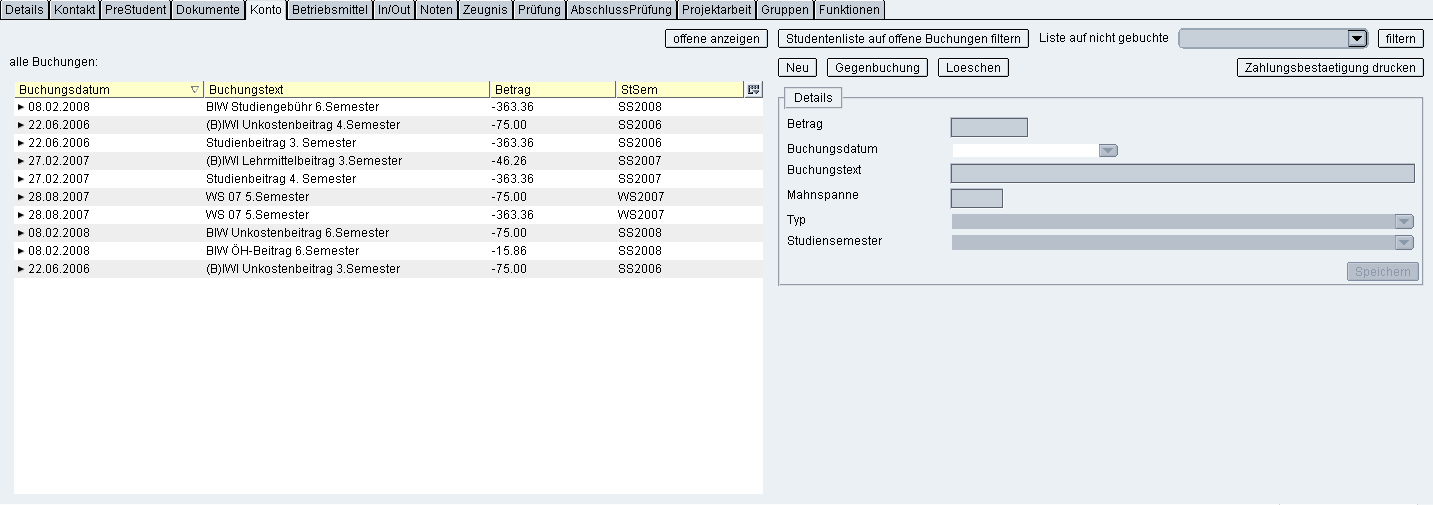
\includegraphics[width=0.75\textwidth]{FAS_Konto1.png}
	\caption{Die Karteikarte Konto}
	\label{Konto1}
\end{figure}
Die Karteikarte besteht aus folgenden Teilen (siehe Abbildung \ref{Konto1}):
\begin{itemize}
	\item Listenfeld: In diesem Anzeigefeld werden die ausgew�hlten Buchungen angezeigt.
	\item Details: Im Details-bereich k�nnen die Buchungsdaten eingegeben und ver�ndert werden.	
	\begin{itemize}
		\item Betrag: Der Buchungsbetrag wird bei einer Belastung negativ eingegeben.
		\item Buchungsdatum: Datum der Belastung oder Bezahlung.
		\item Buchungstext: Kurze Beschreibung der Buchung. (z.B.: BIF Studiengeb�hr 3.Semester)
		\item Mahnspanne: Zeitspanne in Tagen nach eine Mahnung erfolgt.
		\item Typ: Auswahl der Art der Buchung. Zur Auswahl stehen z.Z. \textsl{Kaution}, \textsl{Studiengeb�hr}, \textsl{Lehrmittelbeitrag}, \textsl{sonstiges} und \textsl{Unkostenbeitrag}
		\item Studiensemester: Das Studiensemester in dem bzw. f�r das eingezahlt oder belastet wurde.
	\end{itemize}
	\item Buttons:
	\begin{itemize}
		\item offene anzeigen/alle anzeigen: Schaltet die Anzeige im Listenfeld um. Steht auf dem Button \textsl{offene anzeigen} schaltet ein Knopfdruck auf die Anzeige der offenen Buchungen des Studenten um, steht \textsl{alle anzeigen} wird auf die Anzeige aller Buchungen geschaltet. Dadurch ergibt sich, da� auf dem Button immer das Gegenteil der zeitgleichen Anzeige im Listenfeld steht. Ob gerade alle oder nur die offenen Buchungen angezeigt werden, steht links oberhalb des Listenfelds.
		\item Liste auf nicht gebuchte (Typ) filtern: Wird der Button \textit{filtern} geklickt, werden im Listenfeld 2 alle Studenten der  Ausfwahl (z.B. Semester eines Studiengangs) aufgelistet, bei denen im ausgew�hlten Semester keine Buchung  des ausgew�hlten Typs vorhanden ist.
		\item nicht gebuchte Studiengebuehr: Liefert alle Studenten, die noch keine Belastung der Studiengeb�hr im aktuellen Semester haben.
		\item Neu: Beginn einer neuen Eintragung.
		\item Gegenbuchung: Legt eine Gegenbuchung zu einer im Listenfeld markieren Buchung an.
		\item Loeschen: Entfernen einer markieren (Gegen-)Buchung.
		\item Zahlungsbestaetigung drucken: Ausdrucken einer Zahlungsbest�tigung einer markierten Zahlung.
	\end{itemize}
\end{itemize}
\achtung{\textbf{Wichtig} Bei der Auswahl des Typs wird, sofern das \textit{Betrag}-Feld noch leer ist, dort ein default-Wert (z.B. 363.36 bei Typ Studiengeb�hr) eingef�gt. \\
Zu beachten: Da dies nur geschieht, wenn das \textit{Betrag}-Feld leer ist, wird der Betrag bei einer Fehlerkorrektur des Typs \textbf{nicht} automatisch ge�ndert, sondern mu� manuell �berschrieben werden!}\\

\info{�ber den Men�punkt Einstellungen->\textit{Buchungen auf Studiengang filtern} kann umgeschaltet werden, um alle Buchungen des Studierenden anzuzeigen bzw nur die Buchungen die den aktuellen Studiengang betreffen.}
